\label{chap:problem_formulation}
This chapter provides a problem formulation for self-aware exascale systems by asking three central questions. From there we will put forth a foundation toward solving these questions.

\section{Open Questions}
%{
    There are number of open questions regarding exascale systems. In this section we briefly highlight each and in the subsequent section provide answers toward them. The first open question is how to monitor, make decisions, and control the hardware and software aspects of a exascale system efficiently. Exascale systems present a challenge not found in current systems. They are massive in terms of scale and may consist of thousands of cores, will reach unparalleled energy consumption rates, and cores will not necessarily all have the same capabilities. The second question is how to manage conflicting goals, such as, how to maximize performance while adapting for energy. In exascale systems this problem is burdened by the distributed nature of the control hierarchy where localized job scheduling will no longer suffice. The third question is how to demonstrate a self-aware adaptation strategy for an exascale architecture when to date no architectures have been fabricated; and all are currently in the process of research and development.
%}

\section{Solution Methodology}
%{
    To answer the first question, an exascale architecture such as the TEA will need to support a number of hardware features to enable monitoring within a block as will be discussed detail in Chapter~\ref{chap:requirements}. From there a system runtime will need to make intelligent decisions to control various hardware features within the architecture to reduce energy consumption. This will take the form of clock rate adjustments and clock gating/power gating of components, as well as, bandwidth tapering. From a software decision perspective, a runtime will also need to schedule tasks and move aggregated data distilled from information collected via monitoring the system. We mentioned briefly that this forms the basis for an ODA loop. We foresee each block within the system having some independent ODA loop for localized decisions. Figure~\ref{fig:ODA-TEA} shows at a high level how we foresee the mapping of an ODA mechanism to our TEA. A CE will implement an ODA loop for self-adaptation. Information will come from various hardware and software mechanisms within the system and goals will come from the user or program. And finally, various actions will occur in the form of adjustments to hardware state or some type of software based change (e.g. a goal adjustment).

    \begin{figure}[htb!]
        \centering
        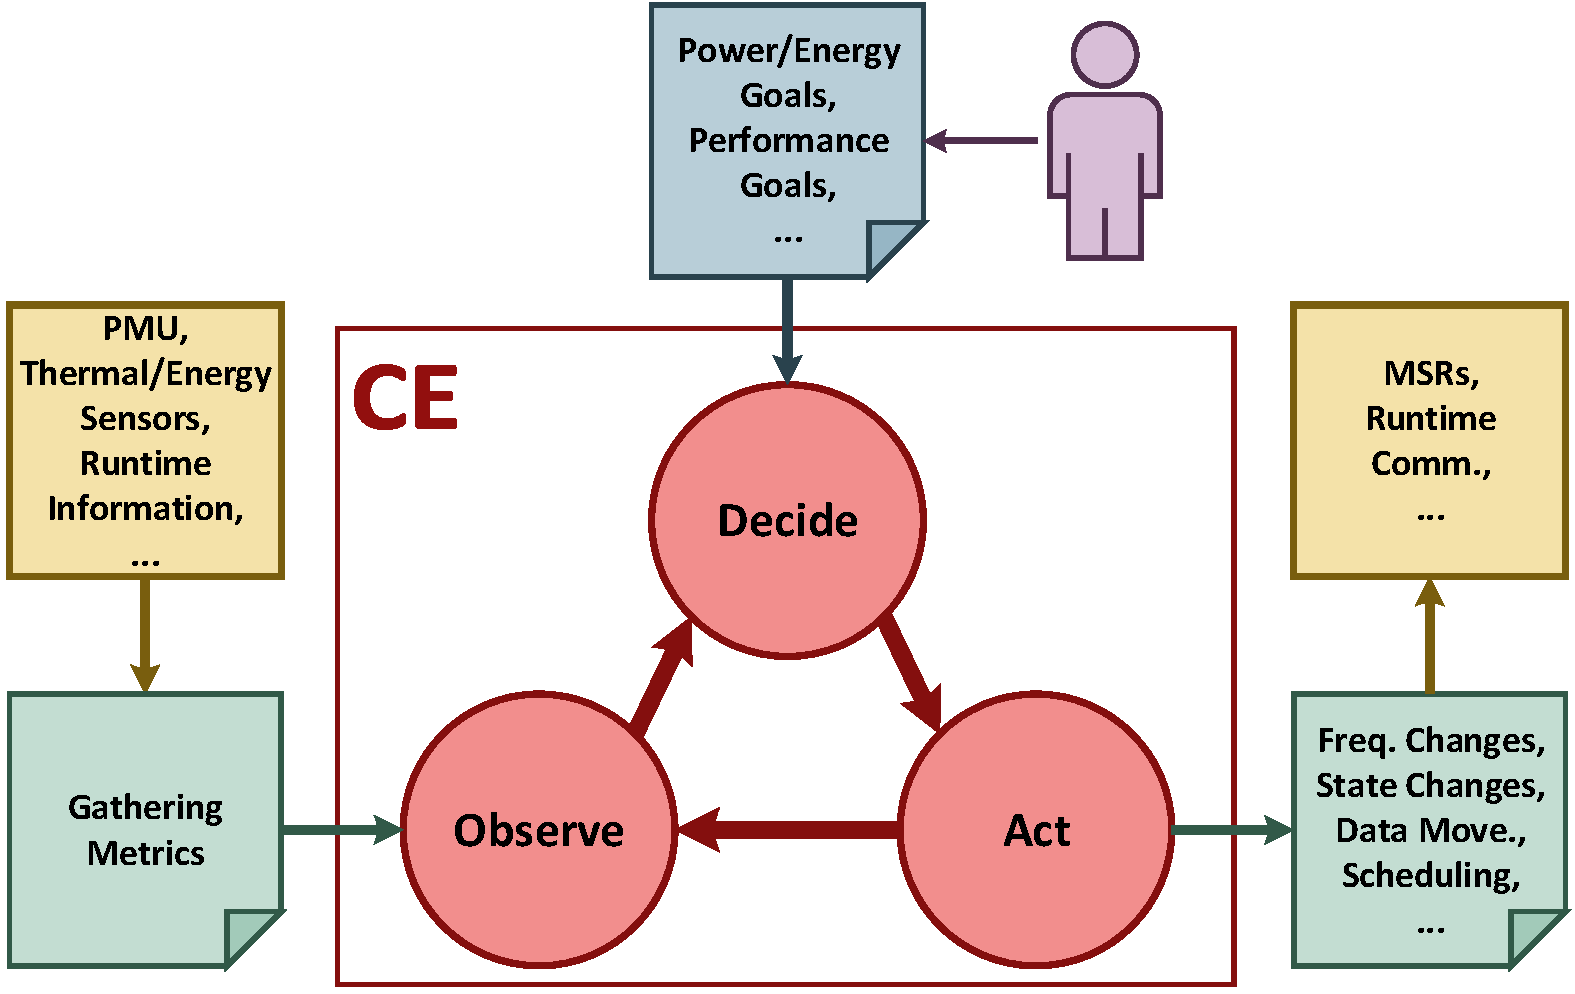
\includegraphics[width=0.9\textwidth]{Fig/ODA_loop_TG.pdf}
        \caption[Mapping our TEA to an ODA Mechanism]{Mapping our TEA to an ODA Mechanism}
        \label{fig:ODA-TEA}
    \end{figure}

   To answer the second question, it is important to recognize that exascale architectures are burdened with a more complicated decision making process than what is typically seen within current generation systems. Exascale systems must adapt to minimize energy, maximize performance, and to be reliable at the very same time. There are two key challenges: (1) conflict resolution, and (2) achieving multi-dimensional efficiency~\cite{Hoffman2013}. As we stated previously, this is an open research problem that has yet to be solved in the current state of the art~\cite{SalehieEtAl2009}. Multi-variable problems are inherently difficult because the search space is too large to do an exhaustive search, and an optimal solution is not known ahead of time (or possibly even the set of actions toward an optimal solution). In exascale architectures, the problem is even further compounded by the hierarchical and complex nature of the system, as well as, because a local control engine will not have complete system information and thus local decisions may not meet overall system goals. We foresee the need for a distributed control in exascale architectures, as well as, a need for a system model. Ultimately whether the solution lies in machine learning or some other type of decision making process is currently unknown. It is worth noting that whatever the mechanism, it needs to operate in real time and be applicable to general workloads.

   To answer the third question, at a high level, we will implement and demonstrate adaptation within our simulation framework, SAFE, as discussed in Chapter~\ref{chap:framework}. This incorporates monitoring and decision making processes. As we will discuss in Chapter~\ref{chap:requirements}, much of the monitoring will be enabled via the architectural features found within the TEA. The implemented features of the TEA within SAFE provide a basis for monitoring the hardware aspects of the TEA, as well as, for modifying the state of components.
%}
